This research aims to identify attack traffic accurately, even when attack traffic dominates benign traffic, by utilizing a large-scale dataset. Besides, we seek to develop a compact model that performs efficiently without requiring extensive computational resources. Additionally, the study focuses on the ability to selectively forget sensitive data whenever needed, ensuring enhanced data security and privacy. Figure-\ref{fig1} illustrates the detailed architecture of the proposed model, DiRLU. The process begins with IoT devices generating network traffic data. This data then goes through preprocessing and feature extraction using engineering techniques. The processed data was split into three portions for training, testing, and validation. In the modeling stage, we use reinforcement learning methods such as A2C, Q-learning and Meta-RL. A feature unlearning module works with these RL models to selectively remove sensitive or outdated features from the system. To make the trained model lighter, we apply knowledge distillation. The distilled model then produces the output (attack or benign). Using XAI (LIME), we explain the model’s decisions so they are transparent and trustworthy. Finally, performance metrics are used to evaluate the effectiveness of the models and to measure the effect of the model.

The following sections provide a detailed explanation of the various phases of the proposed framework. Since multiple symbols are used in later sections, a list of commonly used symbols is included in table-\ref{symbol_table} to enhance the clarity of this paper.

\begin{figure}[htbp]
  \centering
  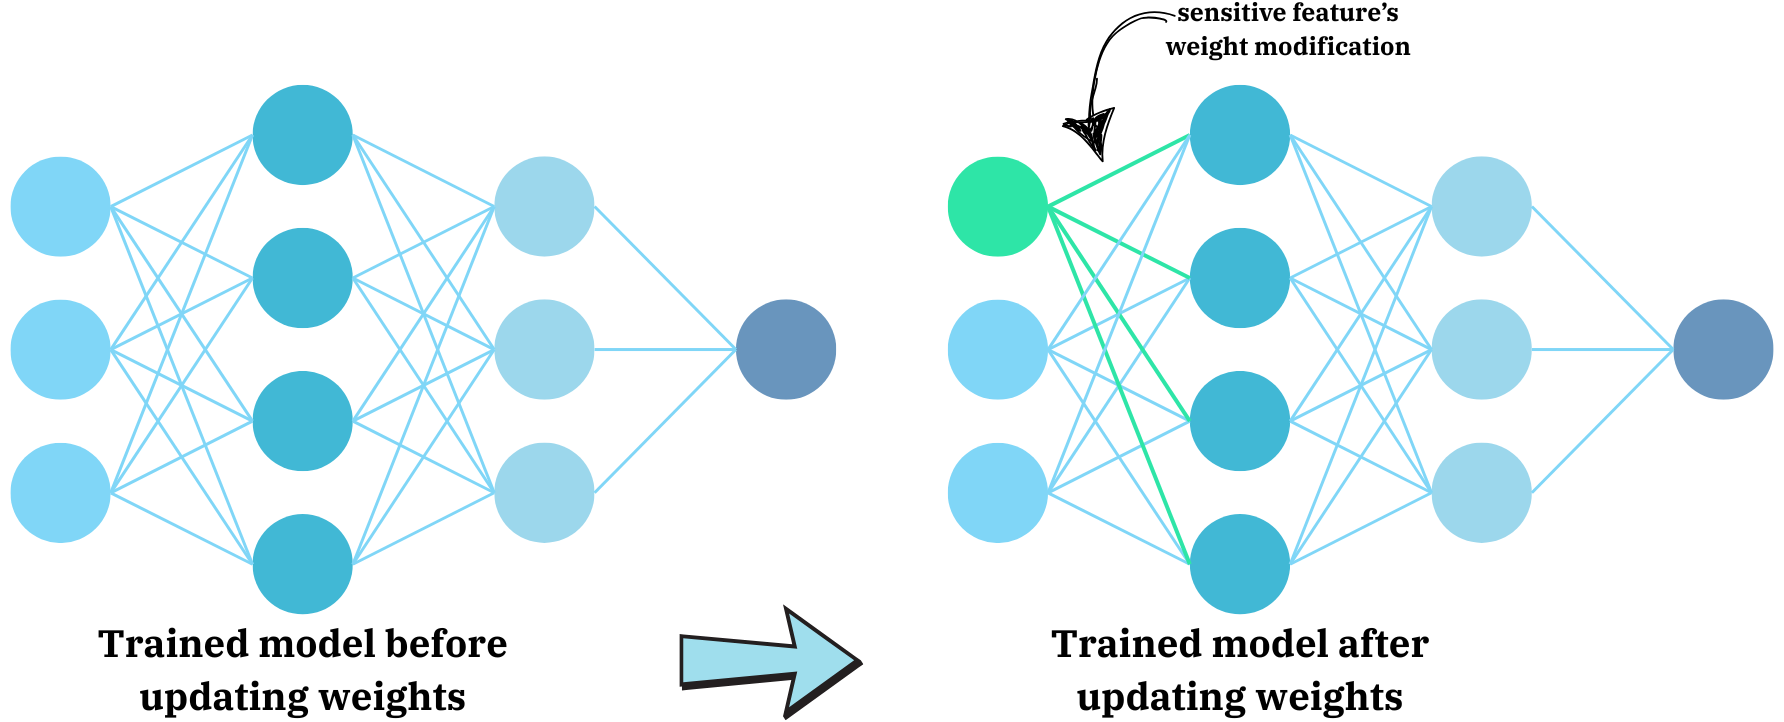
\includegraphics[width=.95\columnwidth]{figure/details_arc2.png}
  \caption{A detailed architecture of the DiRLU framework, where the teacher transfers knowledge to the student via knowledge distillation, integrated with post-hoc feature unlearning module for data privacy also reintroduce unlearned features for scalability}
  \label{fig1}
\end{figure}

%%%%%%%%%%%
\begin{table}[!ht]
    \centering
    \caption{Mathematical Symbols for Proposed Architecture}
    \renewcommand{\arraystretch}{0.9} % reduce row height
    \setlength{\tabcolsep}{6pt} % reduce column spacing
    \small % or \scriptsize
    \begin{tabular}{>{\raggedleft\arraybackslash}p{1.5cm} >{\raggedright\arraybackslash}p{10cm}}
        \toprule
        \textbf{Symbol} & \textbf{Description} \\
        \midrule
        \multicolumn{2}{l}{\textbf{Normalization}} \\
        \midrule
        $x$ & Original value of a feature\\
        $x_{\min}$ & Minimum value of a feature in the dataset \\
        $x_{\max}$ & Maximum value of a feature in the dataset \\
        $x'$ & Normalized value after Min-Max scaling \\
        \midrule
        \multicolumn{2}{l}{\textbf{Actor Network}} \\
        \midrule
        $\pi_\theta(a|s)$ & Policy function of the actor network with parameters $\theta$ \\
        $\theta$ & Parameters of the actor network \\
        $L_{\text{actor}}$ & Loss function for the actor network \\
        $A_t$ & Advantage function at time step $t$ \\
        $\alpha$ & Learning rate for the actor network \\
        $\nabla_\theta$ & Gradient with respect to actor parameters \\
        \midrule
        \multicolumn{2}{l}{\textbf{Critic Network}} \\
        \midrule
        $V_\phi(s_t)$ & Value function of the critic network for state $s_t$ \\
        $L_{\text{critic}}$ & Loss function for the critic network \\
        $R_t$ & Expected cumulative reward at time $t$ \\
        $r_t$ & Immediate reward at time step $t$ \\
        $\gamma$ & Discount factor in reinforcement learning \\
        $\beta$ & Learning rate for the critic network \\
        \midrule
        \multicolumn{2}{l}{\textbf{Knowledge Distillation}} \\
        \midrule
        $P_T(i)$ & Soft target probability from the teacher model for class $i$ \\
        $z_i$ & Logit (output) from the teacher model for class $i$ \\
        $T$ & Temperature parameter for softmax smoothing \\
        $P_S(i)$ & Student model’s predicted probability for class $i$ \\
        $y_i$ & Ground truth label for class $i$ \\
        $L_{\text{CE}}$ & Cross-entropy loss for true labels \\
        $L_{\text{KD}}$ & Distillation loss (KL divergence with soft targets) \\
        $L$ & Total loss function\\
        \midrule
        \multicolumn{2}{l}{\textbf{Evaluation}} \\
        \midrule
        $y_i$ & Ground truth label for class $i$ \\
        $\hat{y}_i$ & Predicted probability for class $i$ by the model  \\
        $n$ & The number of samples\\ 
        \bottomrule
    \end{tabular}
    \label{symbol_table}
\end{table}
%%%%%%%%%%%

\section{Data Description}
The BoT-IoT publicly available dataset was built in a real network environment in the Cyber Range Lab of the University of New South Wales (UNSW) Canberra \cite{data_des_1}. The environment was set in such a way that contained both normal and botnet network traffic. In the dataset, normal traffic is dominated by attack traffic. The dataset is heavily imbalanced, which reflects real-world cyberattack scenarios. They captured traffic using Wireshark, and the total size of pcap files is 69.3 GB, with more than 72 million records and 35 features. The Bot-IoT dataset includes different attacks such as DDoS, DoS, OS and Service Scan, Keylogging and Data exfiltration attacks, which are explained in Table-\ref{table_attackName}.

\begin{table}[!ht]
    \caption{Different cyber-attacks listed in the Bot-IoT dataset}
    \centering
    \renewcommand{\arraystretch}{0.9} % tighter row spacing
    \setlength{\tabcolsep}{4pt} % tighter column spacing
    \begin{tabular}{p{4.3cm} p{10cm}}
    \hline \hline
    \textbf{Attack Name} & \textbf{Description}\\ \hline
     
     Denial of Service (DoS) & An attempt to make a machine or network resource unavailable to its intended users\\ 

     Distributed Denial of Service (DDoS) & Multiple compromised systems attack a target, causing denial of service for users\\

     Reconnaissance & Activities aimed at gathering information about a network for planning future attacks\\

     Information Theft & Unauthorized access and retrieval of sensitive information\\

     Data Exfiltration & Unauthorized transfer of data from a computer or other device\\

     OS and Service Scan & This technique reveals systems and open service (HTTP, FTP, or SMTP) vulnerabilities\\

     Keylogging & This is a secret recording of a user’s keystrokes to capture sensitive information\\
     
     \hline \hline
    \end{tabular}
    \label{table_attackName}
\end{table}

In Table-\ref{table_data_des}, we listed all populated features (total 31) along with their description.

\begin{table}[!ht]
    \centering
    \caption{Feature description of the Bot-IoT dataset}
    \renewcommand{\arraystretch}{0.9} % tighter row spacing
    \setlength{\tabcolsep}{4pt} % tighter column spacing
    \begin{tabular}{l l}
    \hline
        \textbf{Feature Name} & \textbf{Feature Description} \\ \hline
        pkSeqID & Packet number \\
        stime & Packet capture start time \\ 
        flgs & Flow state flags seen in transactions \\
        flgs\_number & Numeric num. of flgs\\
        proto & Protocol used in the flow\\
        saddr & Source IP\\
        sport & Source port\\
        daddr & Destination IP\\
        dport & Destination port\\
        pkts & Total packet count\\
        bytes & Total bytes in the flow\\
        state & Packet state\\
        state\_number & Numeric num. of state\\
        ltime & Packet capture last time \\ 
        seq & Packet sequence number\\
        dur & Total duration\\
        min & Minimum duration of aggregated records\\
        max & Maximum duration of aggregated records\\
        mean & Average duration of total time\\
        stddev & Standard deviation of all records\\
        sum & Total duration of all records\\
        spkts & Source to destination packet count\\
        dpkts & Destination to source packet count\\
        sbytes & Byte count of source to destination packets\\
        dbytes & Byte count of destination to source packets\\
        rate & Packets per second in the flow\\
        srate & Packets per second from source to destination\\
        drate & Packets per second from destination to source\\
        attack & Label: 0 for Normal and 1 for Attack\\
        category & Network traffic category\\
        subcategory & Network traffic sub-category\\ \hline
    \end{tabular}
    \label{table_data_des}
\end{table}

\section{Data Pre-Processing}
Data pre-processing is required to ensure that the data fit properly into the proposed model as it standardizes, normalizes, and handles missing values. This alignment optimizes the model performance and accuracy by furnishing data with uniform, high-quality, and ideal inputs. Firstly, we have dropped the \textit{category and subcategory} column as we do not require them for classification. So, out of 35 features, we worked with 33 features; among them, we selected 32 features for further preprocessing. However, the column named \textit{attack} is used for classification.

\subsection{Feature Pruning}
To have a refined and clean dataset for training the model, we removed all missing or nan values. Some of the features didn't even have any values except nan. So, after removing all nan values, we got 27 columns and 15,000,000 rows. The completely empty features are \textit{smac, dmac, soui, doui, sco, }and\textit{ dco}.

\subsection{Label Encoding}
Label encoding is an essential technique for converting category input to numerical values, which makes it suitable for deep learning algorithms. For example,  we transformed the "attack" category, assigning the value 1 for attack and 0 for not attack. We utilized the \textit{LabelEncoder} function from the \textit{sklearn} library. This conversion allows the model to process the categorical data and use them for classification purposes.

\section{Data Split}
Splitting the dataset into a train, validation, and test subset is crucial for training, validating, and testing the model. We have taken 25\% of the total dataset, whereas previous state-of-the-art research has taken only 5\% \cite{n3}. We got 15,000,000 (Fifteen million) data points in 25\% of the whole dataset. We use a random splitting technique to split the dataset into three parts: training, validating, and testing. We took 70\% of data points for training, 10\% for validating \& tuning hyper-parameters, and another 20\% for testing the model. We randomly choose the 70:20:10 (train:test:validation) ratio for splitting the dataset. However, after splitting, we got 10,500,000 (Ten million five hundred thousand) data points for training the model, 1,500,000 (One million five hundred thousand) data points for tuning hyper-parameters \& validating the model, and 3,000,000 (Three million) data points for testing the model's performance.

\section{Data Augmentation}
We have taken 25\% data points from the BOT-IOT dataset, which gives us a total of 15,000,000 rows. Among those rows, we found attack rows 14,992,430 (Fourteen million, nine hundred ninety-two thousand, four hundred thirty) and the remaining 7,570 (Seven thousand five hundred seventy) non-attack rows. The dataset we have chosen for this research is highly imbalanced, and the ratio of attack vs non-attack is 98:2. So, to balance the dataset, we have used a technique called SMOTE.

SMOTE (Synthetic Minority Oversampling Technique) is an oversampling preprocessing technique used to address class imbalances in the dataset \cite{brandt2021comparative}. It generates synthetic data points by selecting a minority class and creating new data points along the line segments, attaching them to their closest neighbors. This method introduces diversity in the artificial samples, helping to create a non-biased dataset. SMOTE has been widely adopted in machine learning applications to enhance classification performance in imbalanced datasets \cite{chawla2002smote}.

\begin{figure}[htbp]
  \centering
  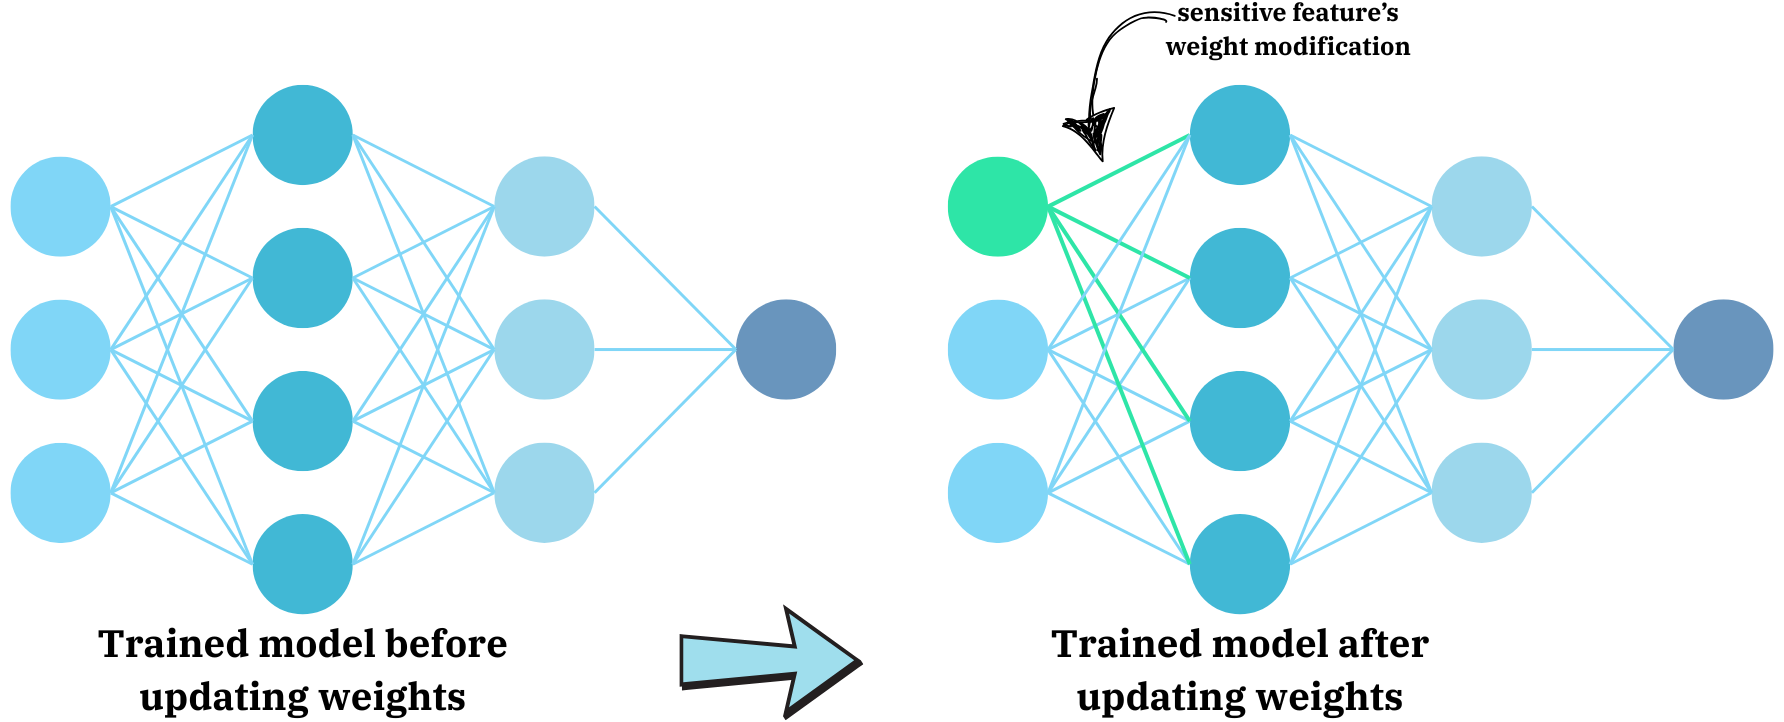
\includegraphics[width=0.65\columnwidth]{figure/fig-2.1.png}
  \caption{Comparison of before and after applying SMOTE}
  \label{fig2}
\end{figure}

After applying smote to the imbalance training dataset, we got 7,035,000 (Seven million thirty-five thousand) rows for the attack class (67\%) and another 3,465,000 (Three million four hundred sixty-five thousand) rows for the non-attack class (33\%), which makes the dataset balanced and non-biased. In Figure-\ref{fig2}, we have represented the ratio and effect of before \& after applying smote.

\section{Data Normalization}
Data normalization is a vital pre-processing technique required for scaling feature values. In the dataset, some feature values are large, and some are very small. Basically, it reshapes numerical values to fit into standard scale values. In this research, we applied deep learning techniques, so we used the Min-Max normalization technique to have values between 0 and 1. Recent studies have proved that Min-Max normalization can significantly improve the accuracy of deep learning models across various applications \cite{deepa2022epileptic}. The Min-Max function normalized the data using equation-\ref{eq:1}.

\begin{equation}\label{eq:1}
x' = \frac{x - x_{\text{min}}}{x_{\text{max}} - x_{\text{min}}}
\end{equation}

In equation-\ref{eq:1}, \(x\) is the original value, \(x_{\text{min}}\) is the minimum \& \(x_{\text{max}}\) is the maximum value in the dataset, and \(x'\) is the normalized value.

\section{Reinforcement Learning}
Reinforcement learning is a type of machine learning where the model learns by interacting with its environment and receiving rewards or penalties for each of its actions, similar to trial and error \cite{RF_IBM}. Unlike traditional deep learning, it does not rely on labeled data but improves through feedback. It is beneficial for solving complex problems like IoT Security \cite{uprety2020reinforcement}.

We have used the actor-critic model because of its enhanced stability compared to traditional reinforcement learning approaches by combining policy optimization with value estimation. In the Fig-\ref{RF_arc}, we represented a simple architecture of the actor-critic model. The actor-critic framework operates through two interconnected neural networks that collaborate to optimize decision-making processes. The actor-network functions as a policy generator, determining which actions to execute based on current states. In contrast, the critic network serves as an evaluator, assessing the quality and long-term value of the actor's chosen actions. During training, the actor adjusts its policy parameters using feedback signals provided by the critic, which simultaneously refines its value estimations based on observed rewards and feedback. This mechanism creates a balanced learning environment by exploring new strategies. The temporal difference error, calculated as the dissimilarity between predicted and actual rewards, is the primary learning signal that guides both networks toward optimal performance \cite{actor_critic_tensorflow}. The actor updates its policy through gradient ascent on expected rewards, while the critic minimizes prediction errors through standard value function approximation techniques. This iterative process continues until convergence, resulting in a robust policy that maximizes cumulative rewards while maintaining stable learning dynamics throughout the training process.

\begin{figure}[htbp]
  \centering
  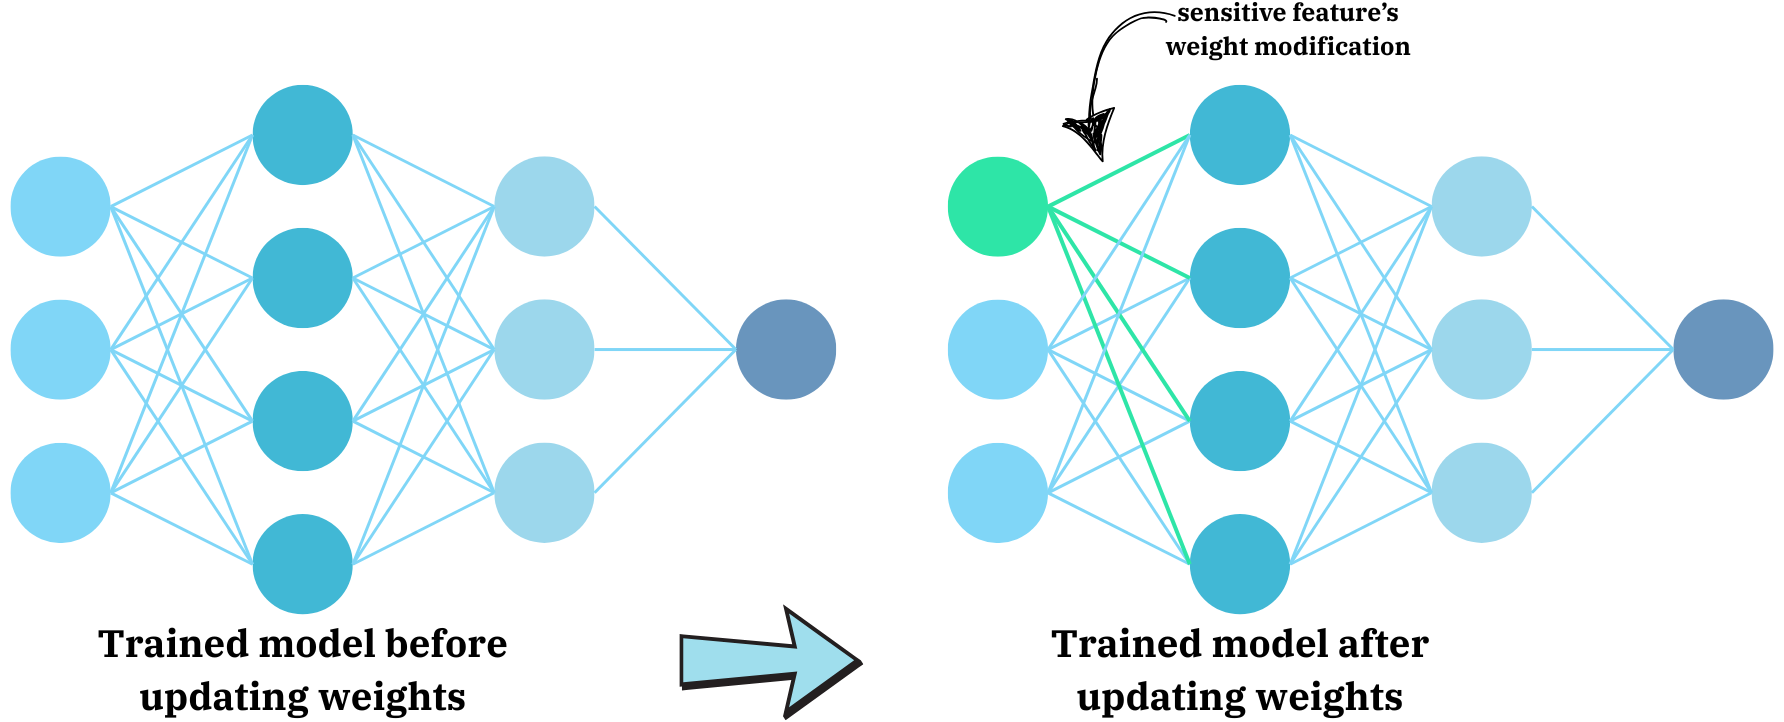
\includegraphics[width=0.60\columnwidth]{figure/RF_arc1.png}
  \caption{Actor-Critic model architecture}
  \label{RF_arc}
\end{figure}

From equations \ref{policy_function}-\ref{critic_update}, we have described the mathematical formulas of the actor-critic model, including both forward propagation and backpropagation update rules.

\begin{equation}\label{policy_function}
\pi_\theta(a|s) = P(a|s; \theta)
\end{equation}
In equation-\ref{policy_function} is Actor Policy Function is shown where the probability of taking action $a$ in state $s$, and $\theta$ denotes the actor network parameters.

\begin{equation}\label{actor_loss}
L_{actor} = -\mathbb{E}[\log \pi_\theta(a_t|s_t) \cdot A_t]
\end{equation}
In equation-\ref{actor_loss} shows the actor loss function, where $A_t$ is the advantage function and $\mathbb{E}[\cdot]$ represents the expected value operator.

\begin{equation}\label{value_function}
V_\phi(s_t) = \mathbb{E}[R_t|s_t]
\end{equation}
In equation-\ref{value_function} shows Critic Value Function where critic parameters is $\phi$, and $R_t$ denotes the expected cumulative reward.

\begin{equation}\label{critic_loss}
L_{critic} = \mathbb{E}[(r_t + \gamma V_\phi(s_{t+1}) - V_\phi(s_t))^2]
\end{equation}
In equation-\ref{critic_loss}, the critic loss function is shown, where $V_\phi(s_t)$ is the state value function, $\gamma$ represents the discount factor, and $r_t$ is the immediate reward at time step $t$.

\begin{equation}\label{actor_update}
\theta \leftarrow \theta + \alpha \nabla_\theta \log \pi_\theta(a_t|s_t) \cdot A_t
\end{equation}
In equation-\ref{actor_update} presents the actor parameter update rule, where $\alpha$ is the learning rate and $\nabla_\theta$ represents the gradient with respect to actor parameters.

\begin{equation}\label{critic_update}
\phi \leftarrow \phi - \beta \nabla_\phi L_{critic}
\end{equation}
In equation-\ref{critic_update}, the critic parameter update is shown, where $\beta$ is the critic learning rate and $\nabla_\phi$ denotes the gradient with respect to critic parameters.

We used actor-critic reinforcement learning in a teacher-student framework for knowledge distillation. In this design, the teacher model has two outputs: the actor makes binary classification decisions using a sigmoid function, and the critic provides continuous value estimates with a linear function. We added an attention mechanism that learns to focus on all the input features with an entropy regularization. We also implemented shared hidden layers, L2 and dropout regularization for better generalization. We use weighted loss functions to handle class imbalance so that underrepresented classes get fair attention during training. Overall, the model jointly optimizes three goals: accurate classification by the actor, precise value estimation by the critic, and balanced attention. This multi-objective setup helps the teacher learn rich representations, which are then passed on to the student model for better learning.

\section{Knowledge Distillation}
Knowledge Distillation (KD) is a model compression technique where a large, complex teacher model transfers its knowledge to a smaller, more efficient student model without significant loss in performance. In this method, the teacher model is initially trained on a dataset, and its output, such as soft probabilities (logits) or intermediate feature representations, is used to assist the student model's training. The student model is optimized using a distillation loss function, which combines standard loss (cross-entropy) with a term encouraging the student to mimic the teacher's outputs. The benefit of the KD is that it reduces the size of networks while maintaining high accuracy and faster inference, making it appropriate for deployment on resource-constrained devices such as mobile phones and edge computing platforms. This technique has been widely adopted in security applications, improving the robustness of AI models against adversarial attacks while maintaining efficiency \cite{gou2021knowledge}. We have used KD to classify malware and begin traffic with low resources. In Fig-\ref{fig4}, we have included an architecture diagram of the knowledge distillation model.

\begin{figure}[htbp]
  \centering
  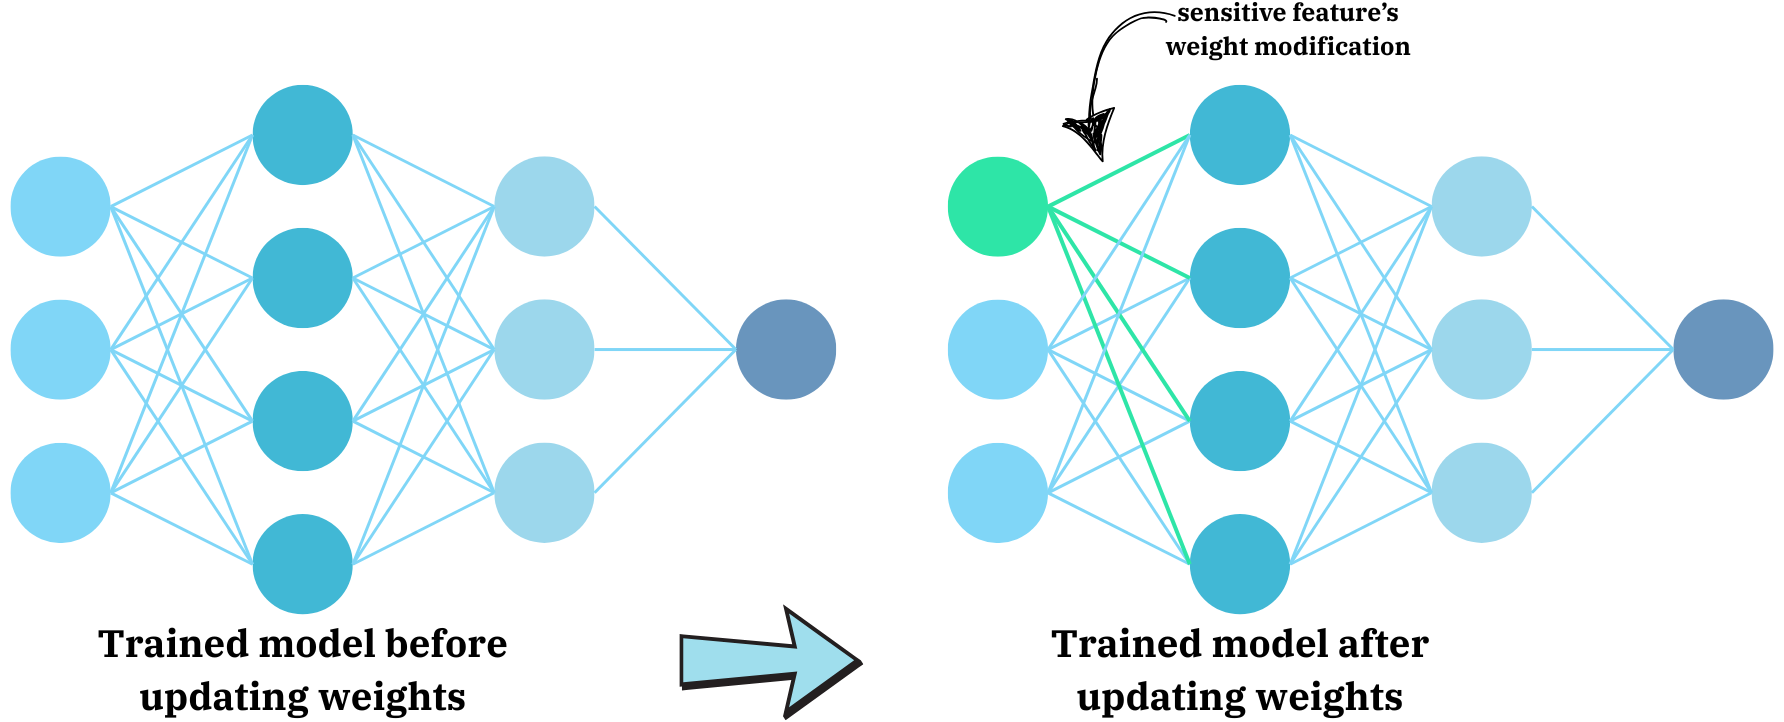
\includegraphics[width=0.65\columnwidth]{figure/fig-4.png}
  \caption{Architecture of knowledge distillation (KD) framework}
  \label{fig4}
\end{figure}

\subsection{Teacher Model}\label{Teacher Model}
We implemented a teacher model within a Knowledge Distillation (KD) framework, where a larger Actor-Critic model transfers its knowledge to a smaller one (student model). The teacher model learns to map input data to output probabilities, which are then used to transfer knowledge to a smaller one. The teacher model produces soft targets $P_T$ by applying a temperature-scaled softmax function to the logits:

\begin{equation}\label{eq:2}
P_T(i) = \frac{\exp(z_i / T)}{\sum_{j} \exp(z_j / T)}
\end{equation}

In equation-\ref{eq:2}, $z_i$ is the logit (output) from the teacher model and 
$T$ is the temperature hyperparameter, which controls the smoothness of the probability distribution. Higher $T$ produces smoother probability distributions.

The teacher model is an attention-enhanced actor-critic architecture. It includes a feature-level attention mechanism that learns from all the individual input features. The attended representation is concatenated with the original input and passed through three shared dense layers with ReLU activation and L2 regularization. The actor's head generates probability scores using a sigmoid activation, while the critic's head estimates value functions using a linear activation. An additional entropy penalty regularizes the attention weights to prevent overly confident focus on a few features. Class weights are dynamically computed and incorporated into the custom binary cross-entropy loss function to address class imbalance. Furthermore, the model uses early stopping on validation accuracy to avoid overfitting and restore the best-performing weights. Training continues until early stopping is triggered, typically within 25–30 epochs. Table-\ref{table_4} provides a complete list of the hyperparameters and their corresponding values used to improve the teacher model's performance.

\begin{table}[!ht]
    \centering
    \caption{Hyperparameters used in teacher model}
    \renewcommand{\arraystretch}{0.9} % tighter row spacing
    \setlength{\tabcolsep}{4pt} % tighter column spacing
    \begin{tabularx}{0.9\columnwidth}{l X} % U
    \hline
        \textbf{Hyperparameter} & \textbf{Value} \\ 
            \hline
            Model & Actor-Critic \\
            Number of Hidden Layers & 3 \\
            Activation Function (Hidden Layers) & ReLU \\
            Activation Function (Actor Output) & Sigmoid \\
            Activation Function (Critic Output) & Linear \\
            Regularization & L2 \& Entropy Penalty\\
            Actor Loss Function & Weighted BSE\\
            Critic Loss Function & MSE\\
            Optimizer & Adam \\
            Epoch Number & Early stopping (max 30)\\
            Batch Size & 512 \\
            Evaluation Metric & Accuracy \& F1 Score \\
            \hline
    \end{tabularx}
    \label{table_4}
\end{table}

To make predictions, probability scores from the actor's head are binarized using a 0.8 threshold, and the F1 score is calculated to evaluate classification performance. This trained teacher model is the foundation for knowledge transfer, guiding the development of a smaller, more efficient student model with similar decision boundaries and attention-driven behaviour.

\subsection{Student Model}\label{Student Model}
A student model is a smaller, more efficient Actor-Critic model trained to replicate the behaviour of a larger and more complex teacher model. It learns using the teacher's softened predictions, allowing it to perform well while being lightweight and faster. With appropriate distillation techniques, student models can accurately mimic the behaviour of the teacher model while drastically reducing the model size and computational complexity, making them ideal for real-time applications in mobile and edge computing \cite{chen2022improved}. The student model mimics the teacher's behavior by optimizing a total loss that combines standard cross-entropy (for true labels) and distillation loss (KL divergence with the teacher's soft targets).\\

The Cross-Entropy Loss for true labels $(L_{\text{CE}})$,

\begin{equation}\label{eq:3}
L_{\text{CE}} = -\sum_{i} y_i \log P_S(i)
\end{equation}

In equation-\ref{eq:3}, $ y_i$ is the ground truth label and $P_S(i)$ is the student model's predicted probability.\\

Distillation Loss (KL divergence with soft targets) $(L_{\text{KD}})$,

\begin{equation}\label{eq:4}
L_{\text{KD}} = T^2 \sum_{i} P_T(i) \log \frac{P_T(i)}{P_S(i)}
\end{equation}

In equation-\ref{eq:4}, $T$ is temperature parameter which controls the smoothness of the probability distribution, $P_T(i)$ is probability output from the teacher model of class $i$ and $P_S(i)$ is probability output from the student model of class $i$.\\

The total loss function $(L)$,

\begin{equation}\label{eq:5}
L = \alpha L_{\text{CE}} + (1 - \alpha) L_{\text{KD}}
\end{equation}

In equation-\ref{eq:5}, $\alpha$ is a weighting factor that balances the cross-entropy loss $L_{\text{CE}}$ and the distillation loss $L_{\text{KD}}$.\\

In this research, the student model consists of a smaller actor-critic model. This student model is smaller and faster than the teacher model. The actor helps predicts the final class (benign or attack), and the critic, which gives a value or score to help guide learning.

We use an attention mechanism to make the model focus on all the input features. These attention-weighted inputs are combined with the original input and passed through two hidden layers. Each layer uses the ReLU activation function, and we apply L2 regularization to reduce overfitting. The final part of the model has two outputs: the actor output uses a sigmoid function for classification, and the critic output uses a linear function to estimate value. We also apply an entropy penalty on the attention weights to ensure the model doesn’t focus too much on only a few features. We train the model using the Adam optimizer with a batch size 32. The actor output is trained with a custom loss function that combines two types of loss: binary cross-entropy, which checks how well the predictions match the actual labels, and KL divergence, which helps the student learn from the soft outputs of the teacher model. We use a temperature value of 2.0 to smooth the teacher’s predictions and an alpha value 0.5 to balance the two losses. For the critic output, we use mean squared error with class weights to handle imbalance in the data. We also include the entropy penalty in the total loss to balance the attention distribution. We use early stopping based on validation accuracy to avoid overfitting, which stops training when the model stops improving. Table-\ref{table_5} provides the list of the hyperparameters and their corresponding values used to improve the student model’s performance.

\begin{table}[!ht]
    \centering
    \renewcommand{\arraystretch}{0.9} % tighter row spacing
    \setlength{\tabcolsep}{4pt} % tighter column spacing
    \caption{Hyperparameters used in student model}
    \begin{tabularx}{0.9\columnwidth}{l X} % Use 'X' for the second column to auto-adjust width
    \hline
        \textbf{Hyperparameter} & \textbf{Value} \\ 
        \hline
        Model & Actor-Critic \\
        Number of Hidden Layers & 2 \\
        Activation Function (Hidden Layers) & ReLU \\
        Activation Function (Actor Output) & Sigmoid \\
        Activation Function (Critic Output) & Linear \\
        Regularization & L2 \& Entropy Penalty\\
        Actor Loss Function & Distillation Loss (CE+KL)\\
        Critic Loss Function & Weighted MSE\\
        Temperature & 2.0 \\
        Alpha & 0.5 \\
        Optimizer & Adam \\
        Epoch Number & Early stopping (max 30)\\
        Batch Size & 512 \\
        Evaluation Metric & Accuracy \& F1 Score \\
        \hline
    \end{tabularx}
    \label{table_5}
\end{table}

%%%%%%%%%%%%%CHANGE KORTE HOBE UPTO THIS POINT%%%%%%%%%%%%%%

\section{Un-learning}
Feature unlearning is a technique designed to remove the influence of specific features from a trained model, ensuring that once removed, those features no longer affect the model’s outputs.
The Price of Forgetting \cite{PriceOfForgetting} introduced an economic approach by offering payments to users for keeping their data, helping servers reduce costs while still respecting user privacy. While our approach plays an important role in meeting privacy regulations, mitigating security risks (such as eliminating data), and enabling efficient model updates without the need for full retraining. Key benefits include regulatory compliance by securely removing sensitive data, cost and time savings from avoiding comprehensive retraining, and greater transparency and trust in AI systems. Recent developments in feature unlearning have introduced methods such as data pruning and selective retraining, which allow models to effectively erase the impact of targeted features while preserving overall performance \cite{zhang2023machine}. In practice, this balance of privacy, efficiency, and model reliability is critical for real-world applications.

The post hoc weight modification technique is used to "forget" sensitive data/features for data security. Instead of retraining the whole model, this technique sets zero weight in the first layer of the specific feature. Post hoc weight modification (PHWM) allows the model to forget specific features by modifying a single weight in the network without costly and time-consuming retraining \cite{hakemi2025post}. In Fig-\ref{PHWM}, we illustrate the process of unlearning.

\begin{figure}[htbp]
  \centering
  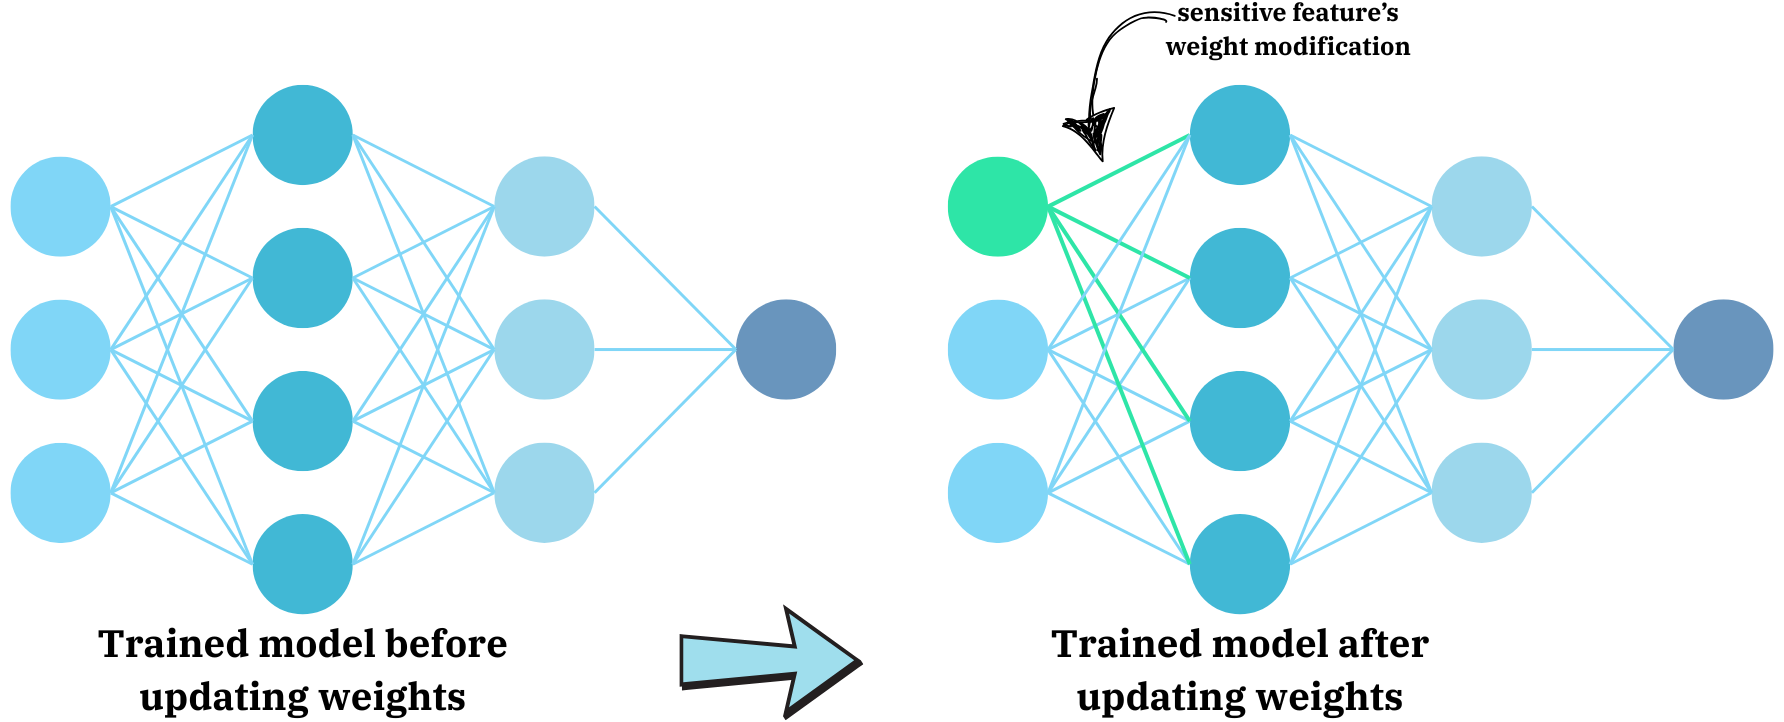
\includegraphics[width=0.95\columnwidth]{figure/deep unlearn.png}
  \caption{Architecture of feature unlearning process}
  \label{PHWM}
\end{figure}

\subsection{Teacher Unlearn}
The procedure of teacher unlearning involves selectively dismissing the second top feature from the dataset that has the most impact on the teacher model. We have used XAI to identify the feature. In this experiment, we have found the second top feature, '\textit{flgs}', for removal from the pre-trained teacher. We removed the feature from the input datasets to ensure the model unlearned them. We also set their corresponding weights in the first layer of the network to zero, preventing them from influencing predictions. After modifying the weight matrix, we reloaded it into the model to ensure the feature was no longer used. To measure the impact of these changes, we re-evaluated the model using accuracy and F1-score. This approach helps improve model interpretability by removing redundant or sensitive features and keeping computations efficient. The approach ensures that the model no longer depends on the removed features, enforcing unlearning at both the data and model levels.

\subsection{Student Unlearn}
The process of student unlearning involves carefully removing the second most influential feature from the dataset that affects the student model. We used XAI to specify the features; in this case, the feature was 'flgs'. The feature was removed from the input datasets to ensure the student model no longer learned or made predictions using them. We set the corresponding weights of the feature in the network's first layer to zero, ensuring the model couldn't rely on them for predictions. After making these changes to the weight matrix, the feature was refilled into the student model to confirm that they were no longer in use. To understand how this influenced the model, we re-evaluated it using accuracy and F1-score. This approach improves the model's interpretability by removing unnecessary or sensitive features while maintaining efficient computations.


\section{Explainable Artificial Intelligence (XAI)}
Explainable AI (XAI) in machine learning and deep learning focuses on making model decisions more transparent and easier to understand. It demonstrates how models arrive at their predictions, which helps build trust and ensures fairness. XAI is also valuable for assessing feature importance by showing how different factors influence model outcomes, an essential step for tuning models and improving performance. By improving interpretability, XAI supports accountability and strengthens the reliability of AI systems. Common approaches include local and global interpretability methods such as SHAP and LIME, which provide insights into both individual predictions and overall model behavior, making it easier to detect biases or errors in decision-making \cite{ribeiro2016should}. Recent work has also applied XAI to anomaly detection in NFV systems, where masked autoencoders are combined with explainability techniques to enhance interpretability and support effective fault localization \cite{AnomalyNFV}.

We used LIME (Local Interpretable Model-agnostic Explanations) to understand how the model makes decisions. LIME explains predictions by generating minor variations around a given data point and analyzing how the model responds. LIME has been applied in diverse machine learning tasks, enhancing model transparency and helping researchers identify potential biases or errors in model predictions \cite{gilpin2018explaining}. A single test instance was randomly chosen, and LIME ranked the top 12 features that influenced the model's conclusion. The explanation mode was set to classification, and discretization was turned off to retain continuous feature representations. The Results were visualized interactively using show\_in\_notebook(). Using LIME, we gained valuable insights into which features played a key role in the model's classification.

\section{Model Evaluation}
In this research, we tested the model's performance using various commonly used metrics, such as accuracy, F1 score, and loss.

Regardless of class, accuracy determines the overall accuracy of the model's predictions and evaluates its performance.

\begin{equation}\label{eq:6}
\textit{Accuracy} = \frac{\textit{TP} + \textit{TN}}{\textit{TP} + \textit{TN} + \textit{FP} + \textit{FN}}
\end{equation}

Precision measures the percentage of the model's predictions that are correct, and recall measures the percentage of relevant data points that the model correctly identified. The mean of precision and recall is the F1 score.

\begin{equation}\label{eq:7}
\textit{Precision} = \frac{\textit{TP}}{\textit{TP} + \textit{FP}}
\end{equation}

\begin{equation}\label{eq:8}
\textit{Recall} = \frac{\textit{TP}}{\textit{TP} + \textit{FN}}
\end{equation}

\begin{equation}\label{eq:9}
\textit{F1 score} = \frac{\textit{2*Precision*Recall}}{\textit{Precision} + \textit{Recall}}
\end{equation}

In equations \ref{eq:6}-\ref{eq:9}, $TP$ denotes true positives, $TN$ denotes
true negatives, $FP$ denotes false positives, and $FN$ denotes
false negatives.

Another evaluation metric, Binary Cross-Entropy ($BCE$) is a loss function used in this paper for binary classification. It measures the difference between accurate labels ($y$) and predicted probabilities ($\hat{y}$). It penalizes inaccurate predictions more when predictions are confident but wrong.


\begin{equation}\label{eq:10}
\text{BCE} = - \frac{1}{n} \sum_{i=1}^{n} \left[ y_i \log(\hat{y}_i) + (1 - y_i) \log(1 - \hat{y}_i) \right]
\end{equation}

In the equation \ref{eq:10}, $y_i$ is the actual label, $\hat{y}_i$ is the predicted probability, and $n$ is the number of samples.

\section{Proposed Algorithm}
In algorithm-\ref{pseudocode}, we explain the pseudocode for the proposed model's architecture in detail. We built the model using Python (v3.12) and different libraries, such as tensorflow, pandas, lime, matplotlib, etc., on Visual Studio Code IDE.

\begin{algorithm*}[!htb]
\caption{Pseudocode of DiRLU}
% --- compact settings ---
\algrenewcommand\algorithmicindent{0.6em}
\algrenewcommand\alglinenumber[1]{\footnotesize #1}
\small % or \scriptsize for even tighter
\resizebox{0.99\linewidth}{!}{%
\begin{minipage}{\linewidth}
\begin{algorithmic}[1]

\Function{Preprocess}{df}
  \State $df_c \gets \textproc{Clean}(df)$; $df_b \gets \textproc{ApplySmote}(df_c)$; $df_{tr}, df_{val}, df_{te} \gets \textproc{Split}(df_b)$
  \State \Return $df_{tr}, df_{val}, df_{te}$
\EndFunction

\vspace{0.4em}

\Function{TrainA2CTeacher}{df\_train}
  \State $teacher \gets \textproc{A2C()}$;\; $w \gets \textproc{CompClsWeights}(df\_train)$
  \While{NOT \textproc{Converged}(teacher, EarlyStop)}
    \State $(x,y) \gets \textproc{Sample}(df\_train)$
    \State $L \gets \textproc{WeightedBCE}(actor(x), y, cls\_weights)+\textproc{MSE}(critic(x), y)$
    \Statex \hspace{1.5cm}$+ \lambda_{attn}\cdot \textproc{Entropy}(attention)$
    \State \textproc{UpdateA2C}$(teacher,\nabla L,\text{Adam})$
  \EndWhile
  \State \Return $teacher$
\EndFunction

\vspace{0.4em}

\Function{FeatureUnlearn}{model, forgetFeat}
  \State $(W_u, b_u) \gets model.\textproc{GetWeights}(\texttt{first\_dense},\textproc{Index}(forgetFeat))$
  \State $W_v \gets 0.0$; $b_v \gets 0.0$
  \State $model \gets model.\textproc{UpdateWeights}(\texttt{first\_dense},\textproc{Index}(forgetFeat), W_v, b_v)$
  \State \Return model
\EndFunction

\vspace{0.4em}

\Function{DistillToStudent}{teacher, df\_train, T}
  \State $student \gets \textproc{A2C()}$; $cls\_weights \gets \textproc{ComClsWeights}(df\_train)$
  \State $t\_probs \gets \textproc{Softmax}(teacher(df\_train)/T)$
  \While{NOT \textproc{Converged}(student, EarlyStop)}
    \State $(x, y) \gets \textproc{Sample}(df\_train)$
    \State $L \gets \alpha \cdot \textproc{CE}(student(x), y) + (1-\alpha) \cdot T^2 \cdot \textproc{KL}(student(x)/T,\ t\_probs)$
    \Statex \hspace{1.5cm}$+ \textproc{MSE}(critic(x), y) + \lambda_{attn} \cdot \textproc{Entropy}(attention)$
    \State \textproc{Step}(student, $\nabla L$, Adam)
  \EndWhile
  \State \Return $student$
\EndFunction

\vspace{0.4em}

\Function{RestoreFeatures}{model, forgetFeat}
  \State $(W_v, b_v) \gets \textproc{SavedWeightsBiases}(\texttt{first\_dense},\textproc{Index}(forgetFeat))$
  \State $model \gets model.\textproc{UpdateWeights}(\texttt{first\_dense},\textproc{Index}(forgetFeat), W_v, b_v)$
  \State \Return model
\EndFunction

\vspace{0.4em}

\State $df_{tr}, df_{val}, df_{te} \gets \Call{Preprocess}{df}; teacher \gets \Call{TrainA2CTeacher}{df_{tr}}$
\State $student \gets \Call{DistillToStudent}{teacher,\ df_{tr},\ T}$

\vspace{0.2em}

\State $base\_models (\mathcal{B}) \gets [teacher,\ student]$
\State $unlearn\_models (\mathcal{UL}) \gets [\,]$
\State $restore\_models (\mathcal{RE}) \gets [\,]$

\vspace{0.2em}

\ForAll{$m \in base\_models$}
  \State $unlearn\_models \gets \Call{FeatureUnlearn}{m,\ df_{fg}}$
\EndFor

\vspace{0.2em}

\ForAll{$m\_ul \in unlearn\_models$}
  \State $restore\_models \gets \Call{RestoreFeatures}{m\_ul,\ df_{fg}}$
\EndFor

\vspace{0.2em}

\State $all\_models \gets\mathcal{B} \cup \mathcal{UL} \cup \mathcal{RE}$

\ForAll{$x \in df_{te}$}
  \ForAll{$m \in all\_models$}
    \State $\hat{y} \gets \textproc{Predict}(m,\ x)$
    \State $\Call{ExplainWithLIME}{\hat{y}}$
  \EndFor
\EndFor
\State $\textproc{CompareResults}(all\_models)$

\end{algorithmic}
\end{minipage}}
\label{pseudocode}
\end{algorithm*}

To conduct the research, a high-performance workstation was configured with 64GB of RAM, a 3.40GHz processor, and an NVIDIA 12GB GPU running Windows 11. This setup ensured optimal processing and memory capacity for data-intensive tasks.